\chapter[Ferramenta]{Ferramenta e-TAPE}
\label{cap:cap3}
Este trabalho teve como proposta o desenvolvimento de uma aplicação web, chamada e-TAPE, cujo o objetivo consiste em
disponibilizar um ambiente para interação com uma taxonomia para ferramentas de participação eletrônica.

\par
Para desenvolver a aplicação foi adotado o modelo de ciclo de vida incremental, descrito na seção subsequente.

\section {Desenvolvimento}
\label{sec:desenvolvimento}
\par
Segundo \citeonline{sommerville2016software}, o modelo incremental é baseado na ideia de se desenvolver uma aplicação inicial,
realizar a coleta de \textit{feedback} de clientes, usuários e outras pessoas envolvidas, evoluir a aplicação em versões, até que o desenvolvimento dos requisitos levantados seja realizado.

\par
Cada versão entregue da aplicação, deve incorporar novas funcionalidades para melhor atender os requisitos levantados. Geralmente, ainda segundo o autor, as primeiras funcionalidades
implementadas são escolhidas pelo grau de importância para o produto final. Esse modelo permite a avaliação da aplicação em versões iniciais de desenvolvimento, para assim saber 
se os requisitos estão sendo entregues. A figura \ref{fig:modelo-incremental} demonstra a abstração do modelo incremental.


\begin{figure}[!ht]
    \centering
    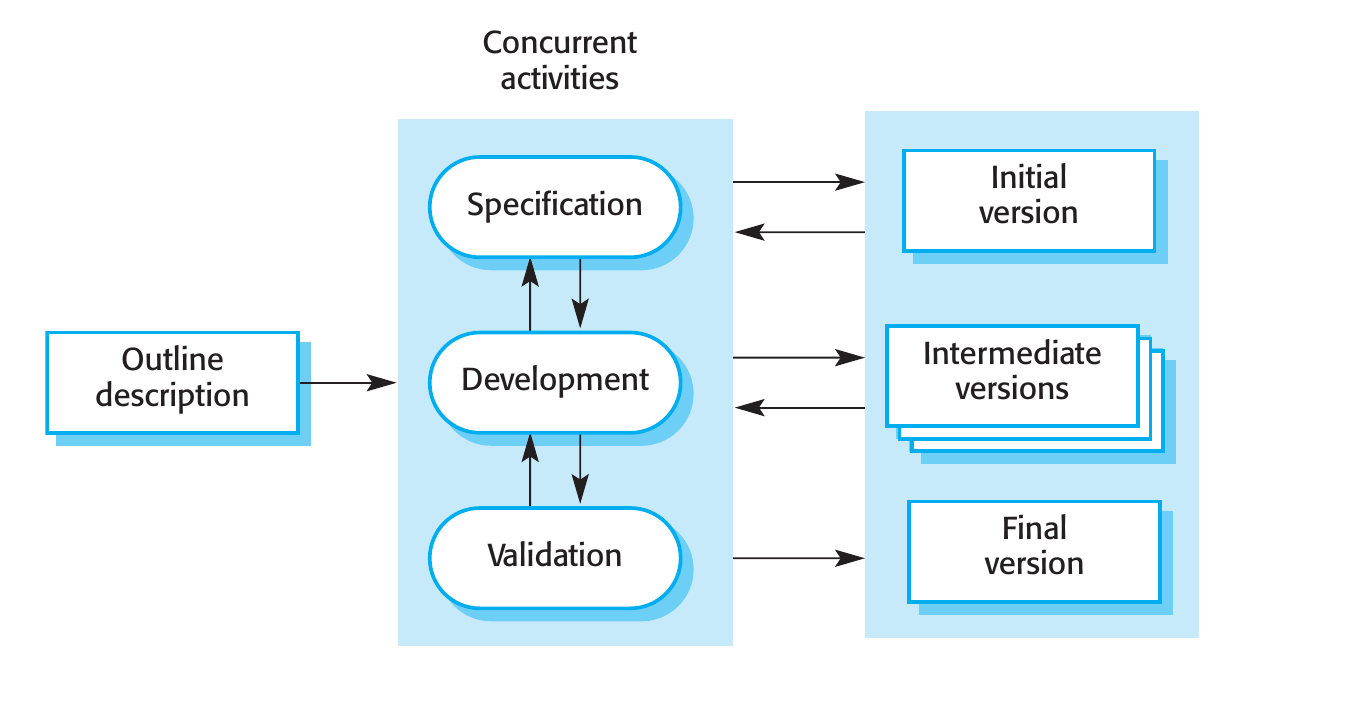
\includegraphics[scale=0.20]{./figuras/modelo_incremental.png}
    \caption{Modelo de desenvolvimento Incremental \citeonline{sommerville2016software}}
    \label{fig:modelo-incremental}
\end{figure}

\par
Para o desenvolvimento da aplicação inicial, foram realizados o levantamento dos requisitos de cliente, a modelagem das entidades e a definição das principais funcionalidades. 

\par
Passada essa primeira fase, houve o detalhamento dos requisitos de sistema, desenho do protótipo inicial e definição dos atores da aplicação.
O documento de requisitos para a aplicação encontra-se no apêndice deste trabalho. 

\par
Finalizada a etapa de projeto, iniciou-se a etapa de implementação. 

A aplicação foi construída utilizando a plataforma de desenvolvimento Node.js. A escolha dessa plataforma justifica-se pelo conhecimento técnico da equipe
responsável pelo desenvolvimento da aplicação e pelo conceito fundamental da plataforma. Node.js é uma plataforma construída sobre o motor JavaScript do 
Google Chrome para facilmente construir aplicações de rede rápidas e escaláveis. Node.js usa um modelo de I/O direcionada a evento não bloqueante que o torna leve e eficiente,
ideal para aplicações em tempo real com grande volume de troca de dados através de dispositivos distribuídos. 
\textit{Node.js} Disponível em: <https://nodejs.org>. Acesso em 01 out. 2018.

\par
Após análises, foi identificada a necessidade da utilização de um banco de dados orientado a documentos para a realizar a persistência dos dados da aplicação. 
Sendo assim, a utilização do banco de dados MongoDB apresentou-se como uma escolha adequada. 
Por se tratar de uma ferramenta \textit{open source}, e por se integrar com a plataforma Node.js, MongoDB atendeu aos requisitos necessários para o desenvolvimento da aplicação.
\textit{MongoDB} Disponível em: <https://mongodb.com>. Acesso em 01 out. 2018.

\par
O \textit{front-end} da aplicação, foi implementado com a utilização do \textit{framework} responsivo Materialize, pois esse, 
mostrou-se uma opção elegante e prática para o desenvolvimento da aplicação. Combinando o Materialize com o \textit{framework} de templates EJS, 
foi possível desenvolver a aplicação de maneira escalável e leve. \textit{Materialize} Disponível em: <https://materializecss.com>. Acesso em 01 out. 2018.
\textit{EJS} Disponível em: <https://ejs.co>. Acesso em 01 out. 2018.

\par
A implementação de ambas visualizações da taxonomia, radial e horizontal, foram implementadas usando D3.js, uma biblioteca JavaScript para a manipulação de documentos 
baseada em dados. \textit{D3js} Disponível em: <https://d3js.org>. Acesso em 01 out. 2018.

\par
O controle de versão da aplicação foi realizado através do sistema de controle de versão Git na plataforma GitLab, \textit{GitLab}. 
Disponível em <https://gitlab.com>. Acesso em 01 out. 2018.

\par
Foi realizado um estudo sobre a análise de usabilidade da aplicação, esse estudo é demonstrado no Capítulo \ref{cap:cap4} deste trabalho.
\newpage

\section{Funcionamento}
\label{sec:funcionamento}
A ferramenta e-TAPE foi desenvolvida como uma aplicação web, e encontra-se disponível em http://taxonopart.hopto.org:3001.
Denomina-se por usuário, a partir deste momento, qualquer pessoa acessando a aplicação. 

\par
Ao acessar o endereço da aplicação, o usuário encontra uma breve explicação sobre o contexto do projeto ao qual ela foi desenvolvida e uma descrição da taxonomia considerando os grupos,
classes e subclasses propostas. É possível obter detalhes, sobre as classes e subclasses, clicando em seus nomes. 

\par
Ao acessar a página Taxonomia, o usuário começa sua interação ativa com a aplicação.
Foram disponibilizados dois modos de visualização da taxonomia: o e-TAPE 360º e o e-TAPE Árvore, ilustrados, respectivamente,
nas Figuras \ref{fig:e-tape360} e \ref{fig:e-tapeArvore}. O usuário pode alterar entre os modos de visualização clicando no botão logo acima da visualização.
O botão pode ser visto na Figura \ref{fig:pag-taxonomia}.

\vspace{1cm}

\begin{figure}[!ht]
    \centering
    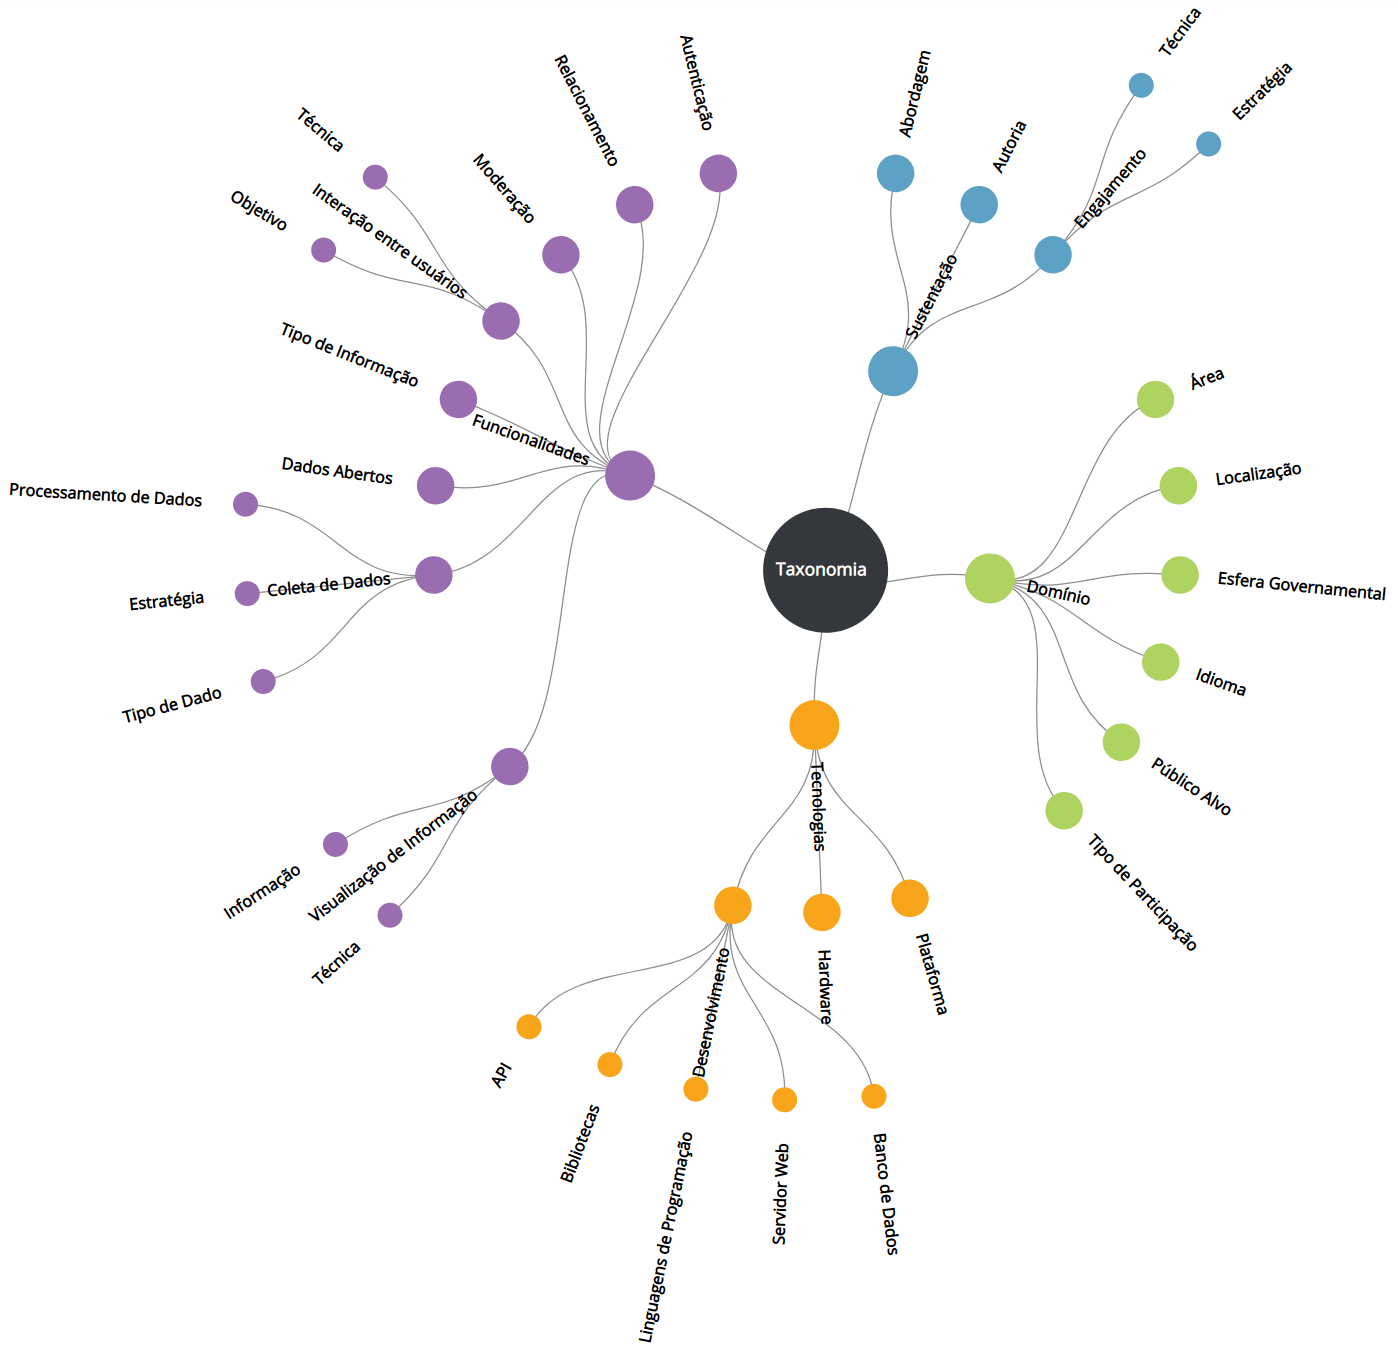
\includegraphics[scale=0.20]{./figuras/taxonomia-cropped.png}
    \caption{e-TAPE 360º}
    \label{fig:e-tape360}
\end{figure}

\vspace{1cm}

\begin{figure}[!ht]
    \centering
    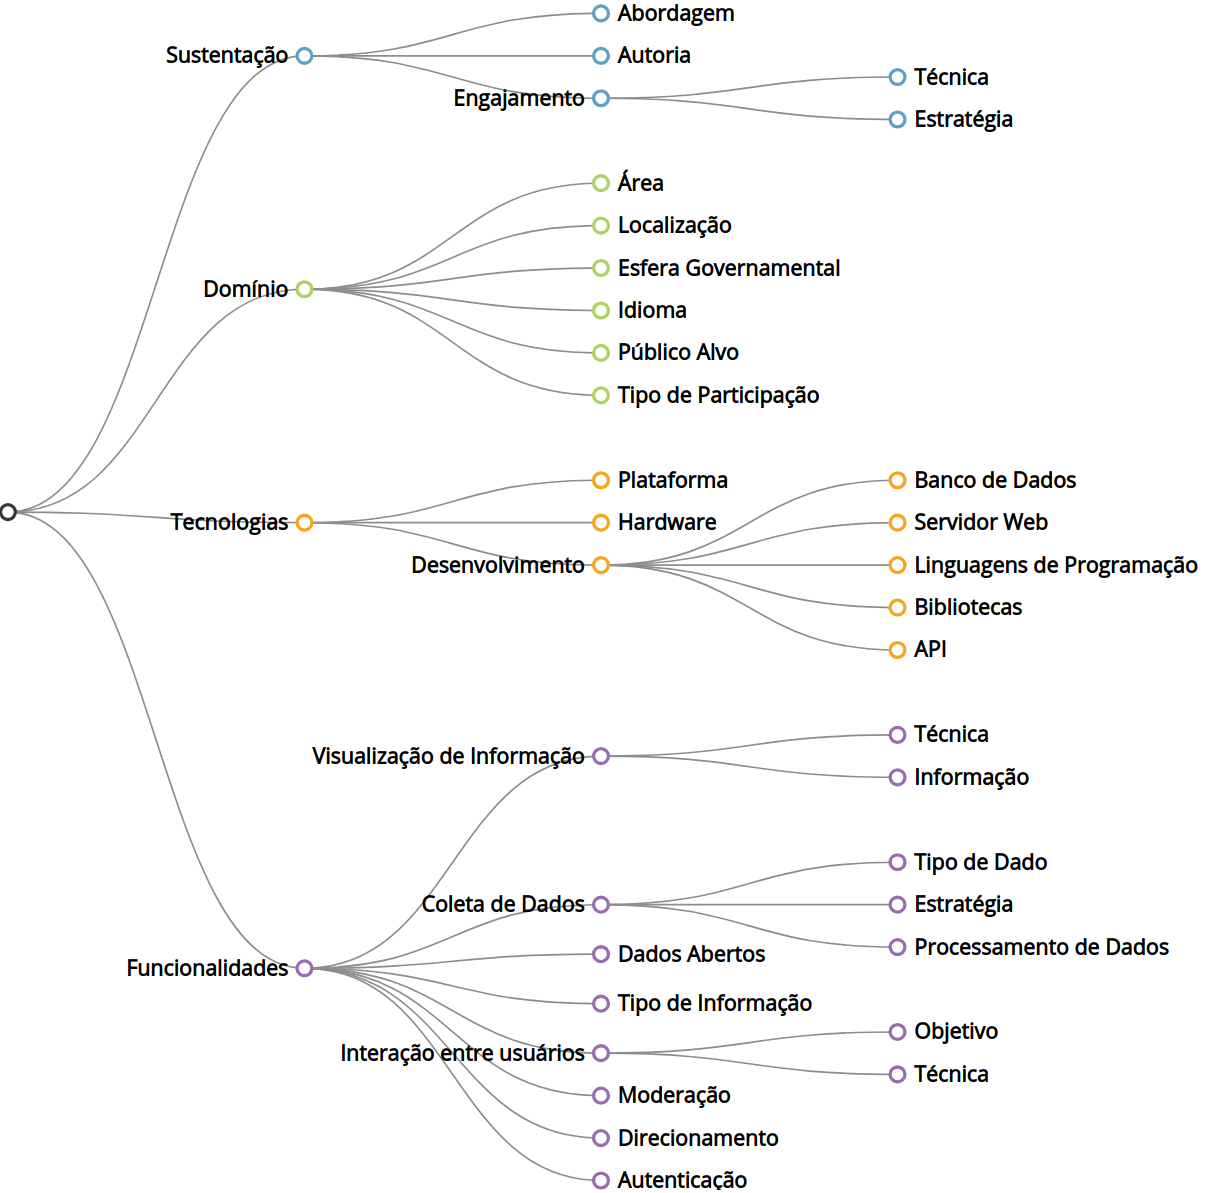
\includegraphics[scale=0.20]{./figuras/taxonopart-horizontal.png}
    \caption{e-TAPE Árvore}
    \label{fig:e-tapeArvore}
\end{figure}
\newpage

\par
Caso queira visualizar uma ferramenta já classificada, o usuário deve utilizar o campo de pesquisa, no canto superior esquerdo da tela Taxonomia.
Conforme o usuário for digitando o nome da ferramenta, o campo sugere ferramentas pelo modo de preenchimento automático. Se o usuário escreveu o nome da ferramenta corretamente, 
e a ferramenta já se encontrar no banco de dados da aplicação, será possível para o usuário clicar no campo com o nome da ferramenta e assim, uma tabela com a classificação da 
ferramenta será mostrada, vide Figura \ref{fig:show-ferramenta}.

\vspace{0.5cm}

\begin{figure}[!ht]
    \centering
    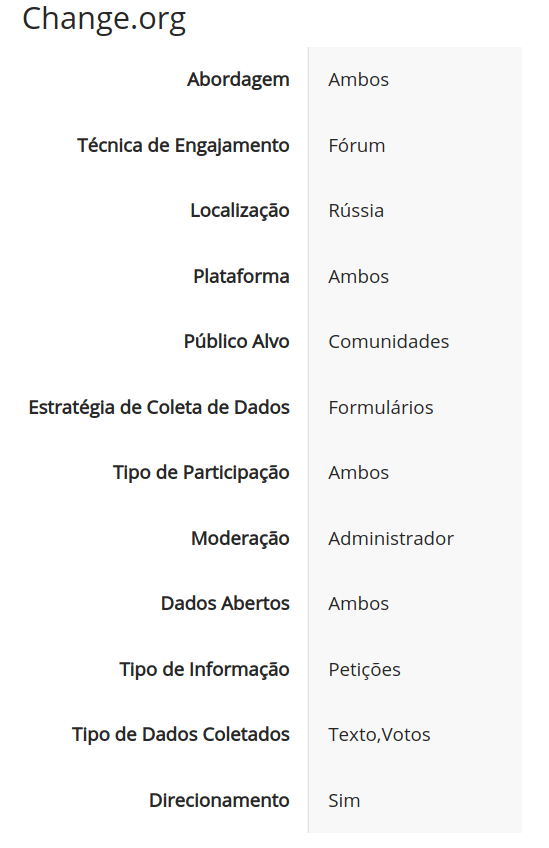
\includegraphics[scale=0.20]{./figuras/show-ferramenta.png}
    \caption{Visualizar ferramenta classificada}
    \label{fig:show-ferramenta}
\end{figure}


\par
Para classificar uma nova ferramenta, o usuário deve clicar no botão com o  sinal de mais, no canto inferior da tela Taxonomia, ilustrada na Figura \ref{fig:pag-taxonomia},
tendo feito isso, o formulário para classificação da ferramenta é exibido, conforme ilustrado na Figura \ref{fig:new-ferramenta}. 

\begin{figure}[!ht]
    \centering
    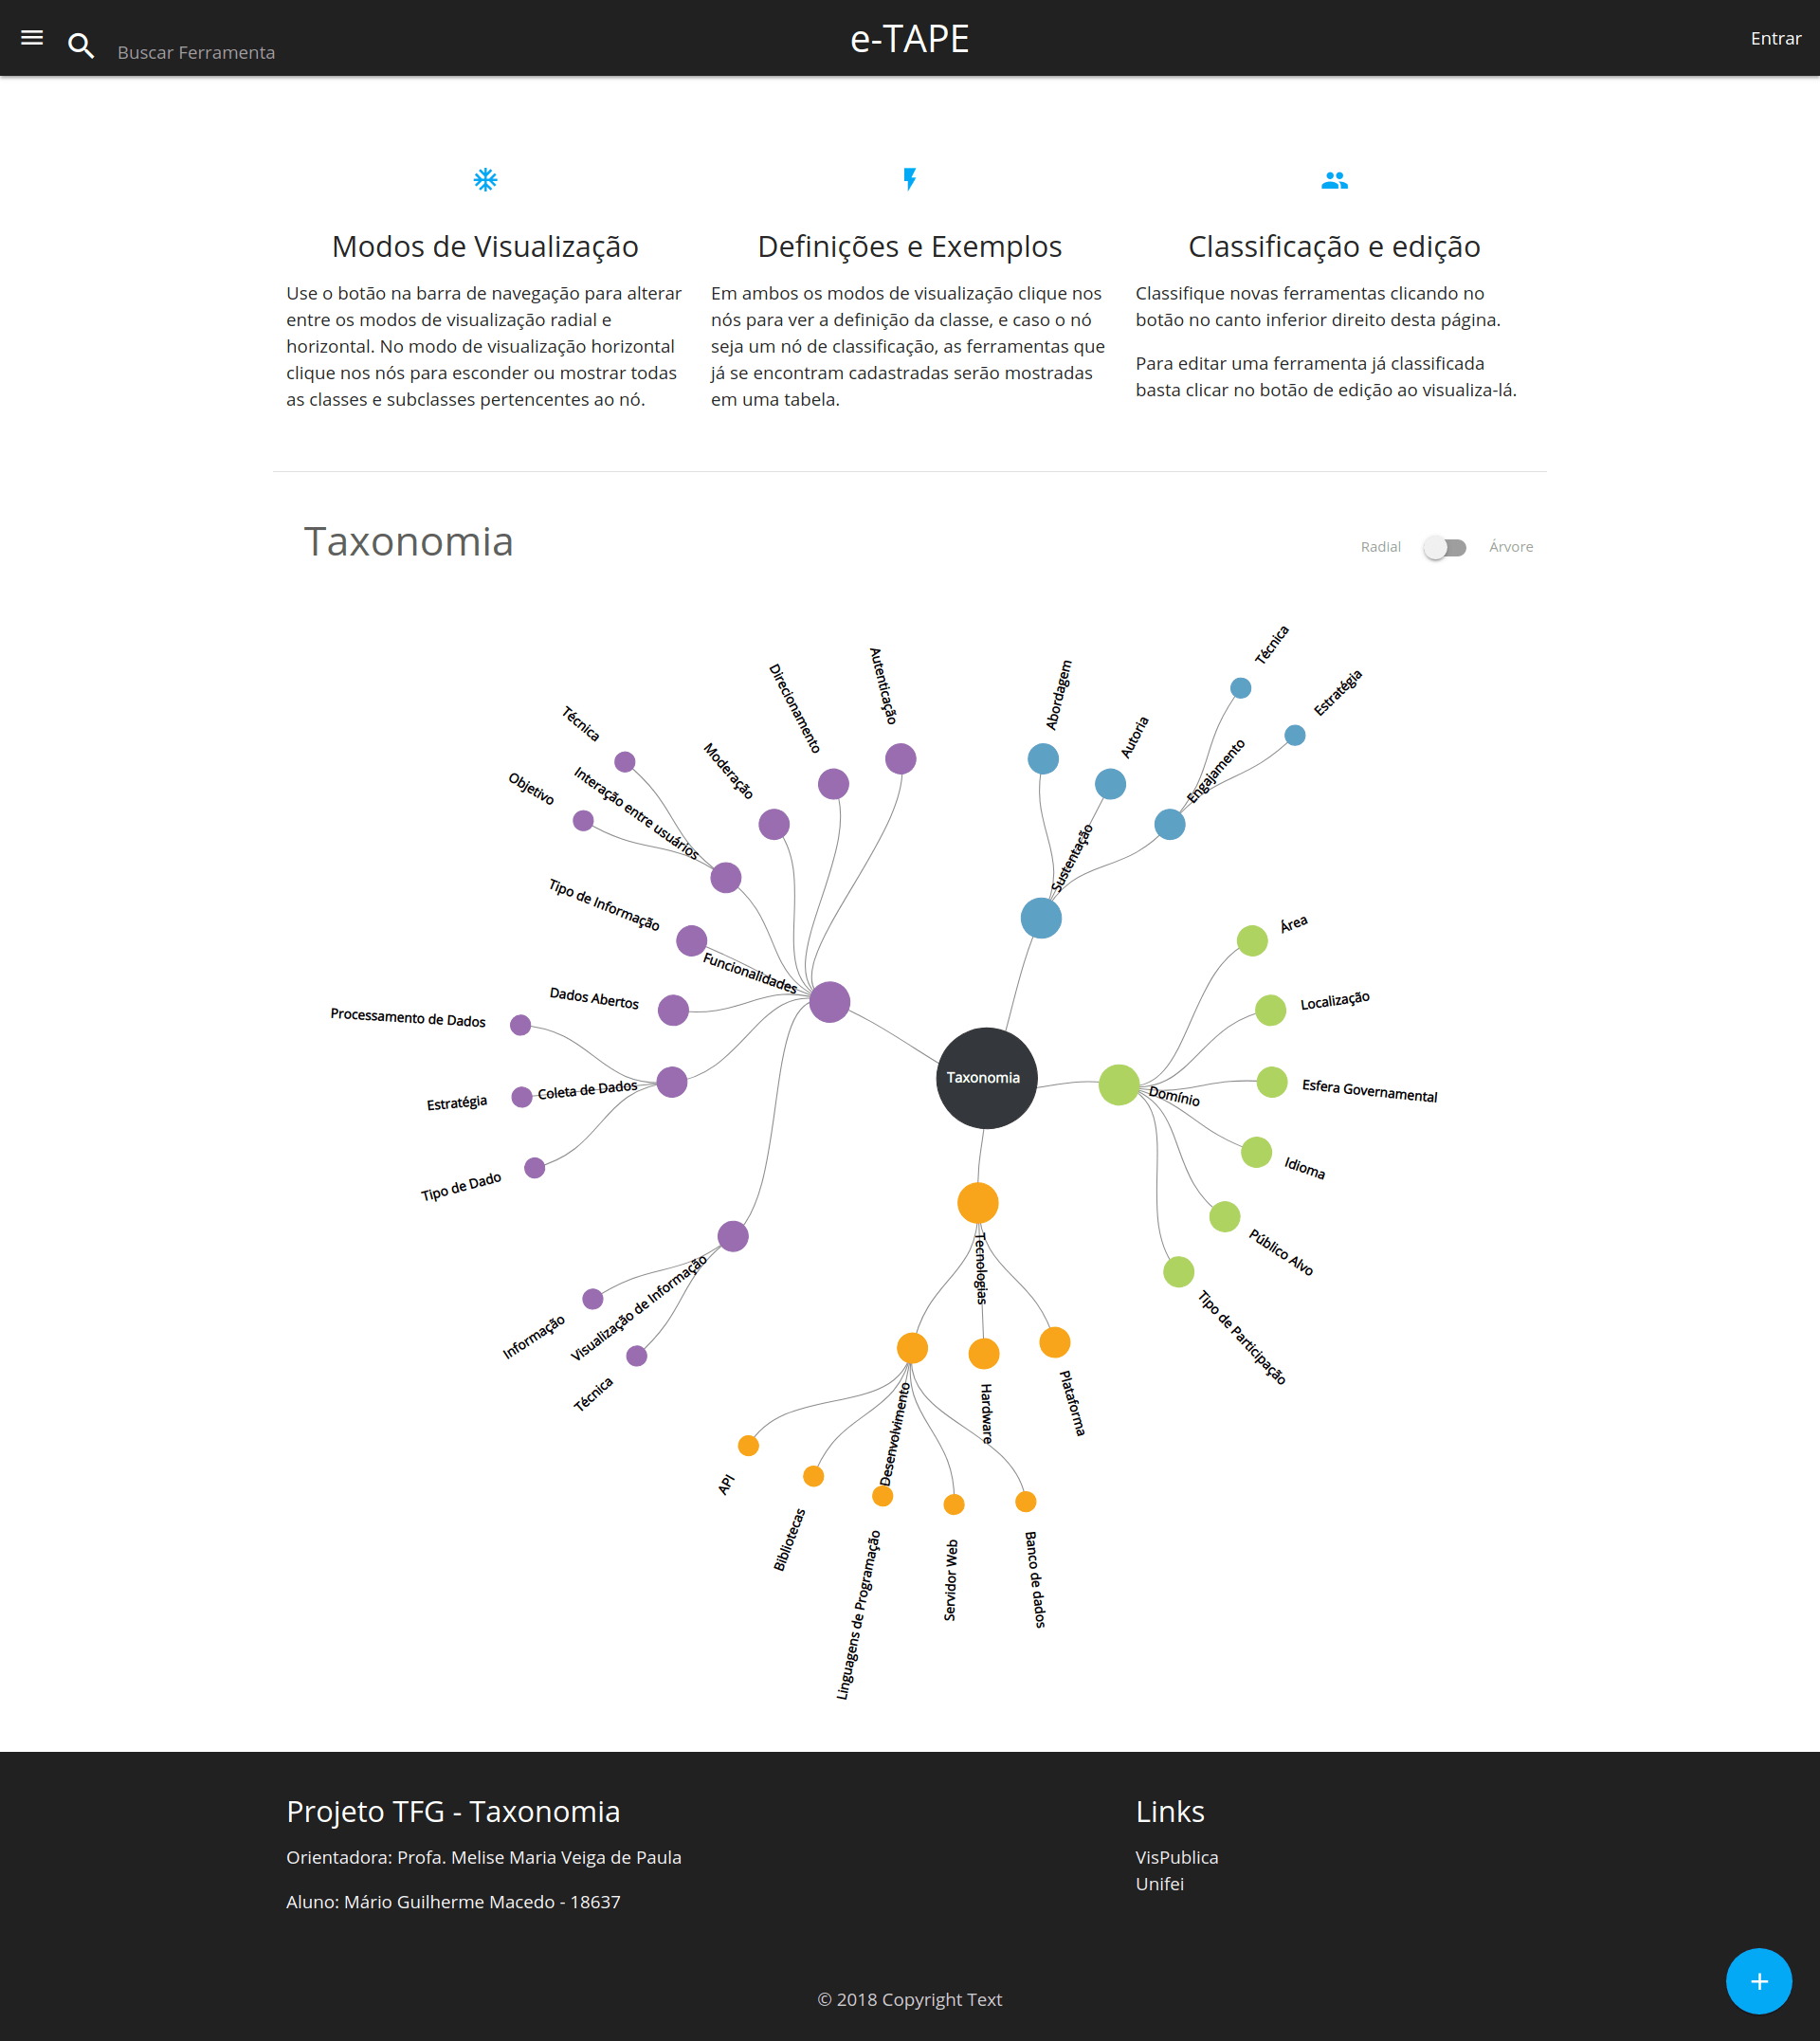
\includegraphics[scale=0.10]{./figuras/pagina-taxonomia.png}
    \caption{Página Taxonomia em e-TAPE }
    \label{fig:pag-taxonomia}
\end{figure}

\par
O formulário de classificação de novas ferramentas foi dividido de acordo com os grupos definidos na taxonomia 
(sustentação, domínio, tecnologias e funcionalidades), sendo o único campo de preenchimento obrigatório, o nome da ferramenta.
Para finalizar a classificação da nova ferramenta o usuário pode a qualquer momento clicar no botão salvar. 

\begin{figure}[!ht]
    \centering
    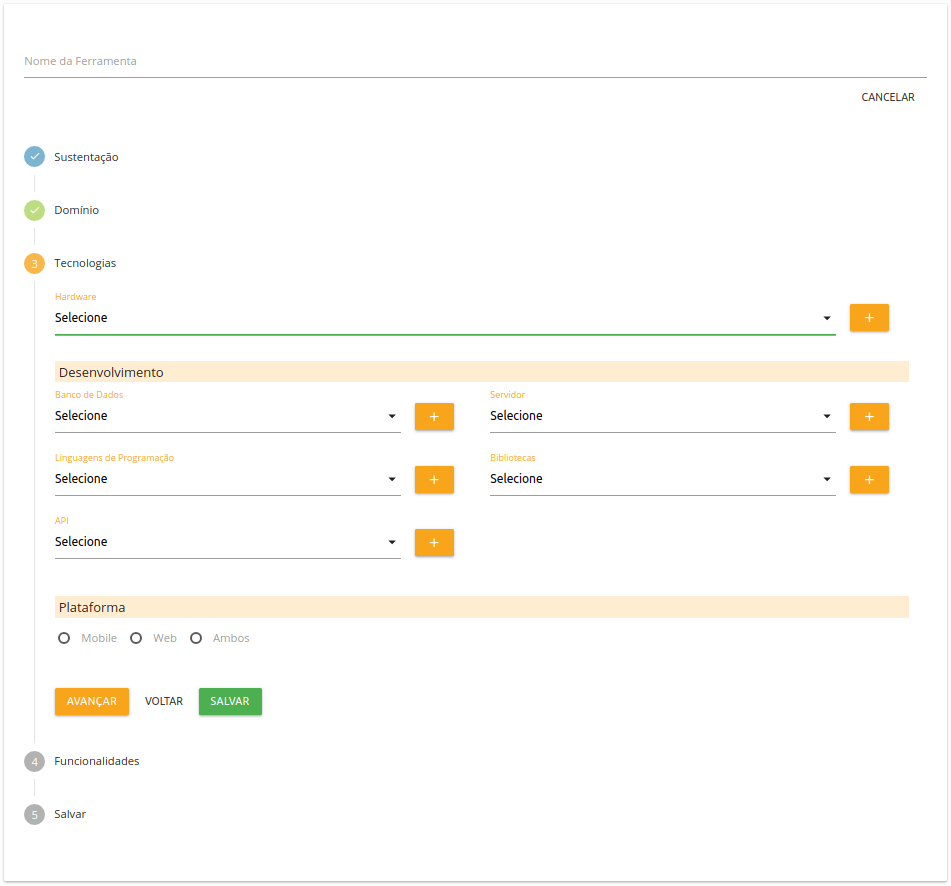
\includegraphics[scale=0.20]{./figuras/new-ferramenta.png}
    \caption{Formulário de classificação ferramentas}
    \label{fig:new-ferramenta}
\end{figure}

\par
Por se tratar de uma ferramenta colaborativa, o usuário é capaz de visualizar e editar qualquer ferramenta já classificada por outros usuários. 
Para fazer isso, o usuário pode usar o campo buscar ferramenta, localizado no canto superior esquerdo da tela, para após  visualizar a ferramenta clicar no botão editar, que 
se encontra no cando superior direito da tabela com os dados de classificação da ferramenta em questão, com isso, os dados da ferramenta selecionada serão inseridos nos
campos do formulário de classificação de ferramentas, previamente demonstrado pela figura \ref{fig:new-ferramenta}. 

\newpage
\par
Ao clicar em algum nó da taxonomia, em qualquer modo de visualização, é exibido um quadro com o nome da classe, sua descrição e todas as ferramentas
com valor de classificação atrelados à classe, ou subclasse em questão. A figura \ref{fig:tabela-ferramentas} demonstra essa ação. 

\begin{figure}[!ht]
    \centering
    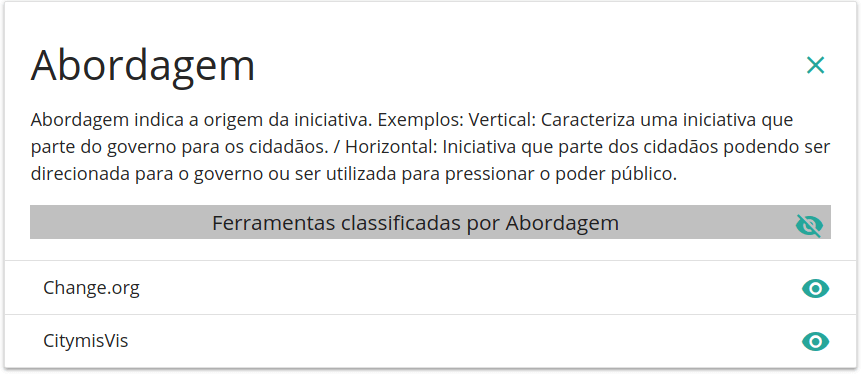
\includegraphics[scale=0.20]{./figuras/abordagem.png}
    \caption{Tabela com ferramentas classificadas segundo Abordagem}
    \label{fig:tabela-ferramentas}
\end{figure}

\section{Evolução da Ferramenta}
\label{sec:evolucao-ferramenta}
Como já abordado no começo da seção \ref{sec:desenvolvimento}, a utilização do modelo interativo de desenvolvimento permite que requisitos sejam propostos e avaliados para serem
implementados em futuras versões.

\par
Algumas funcionalidades já estão previstas para serem implementadas em um futuro próximo, como por exemplo, cadastro de usuários; criação de uma classe de usuários moderadores,
para que ferramentas possam ser editadas de uma maneira moderada; integração com redes sociais e sugestão de evolução da taxonomia. 